\section*{Analiza wielkości wyjaśnień}

W tej sekcji przeprowadzono analizę wpływu wielkości obiektu na wielkość obszaru wyjaśniania wgenerowango przez: LIME, SHAP i GradCAM.
Celem analizy było zobaczenie jak metody radzą sobie z różnymi rozmiarami obiektu.

\begin{figure}[h]
	\centering
	\begin{subfigure}[b]{0.45\textwidth}
		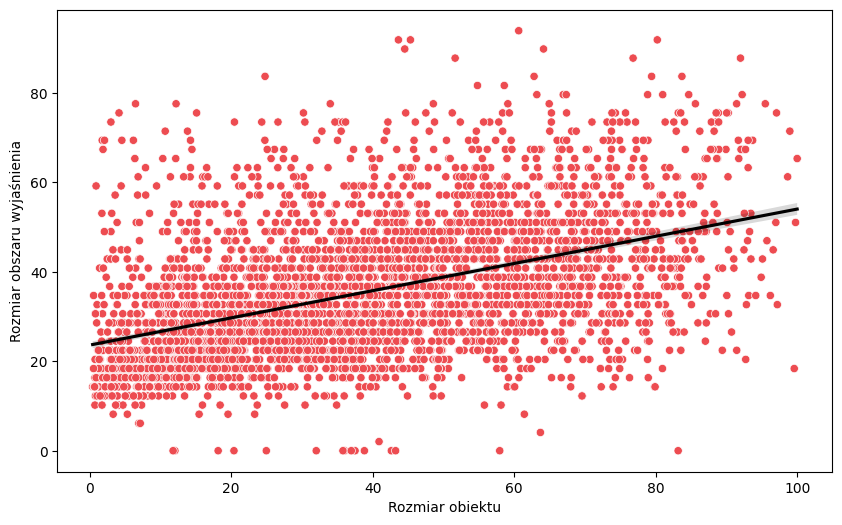
\includegraphics[width=.9\textwidth]{img/size_exp_gradcam}
	\end{subfigure}
	\begin{subfigure}[b]{0.45\textwidth}
		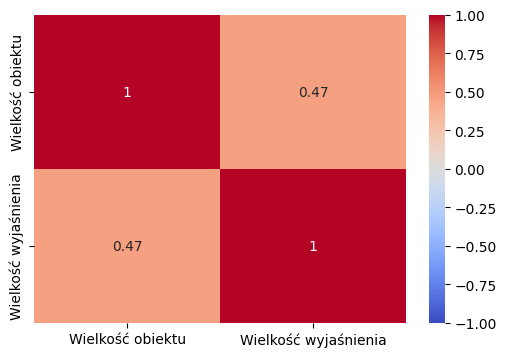
\includegraphics[width=.9\textwidth]{img/size_exp_gradcam_corr}
	\end{subfigure}
	\caption{Zależność między rozmiarem obiektu, a rozmierem obszaru wyjaśnienia GradCAM}
	\label{rys:size_exp_gradcam}
\end{figure}
\begin{figure}[h]
	\centering
	\begin{subfigure}[b]{0.45\textwidth}
		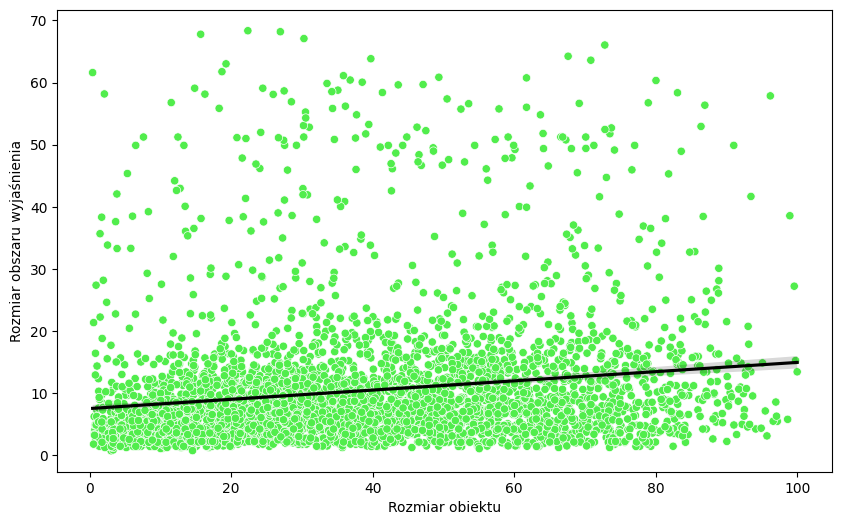
\includegraphics[width=.9\textwidth]{img/size_exp_lime}
	\end{subfigure}
	\begin{subfigure}[b]{0.45\textwidth}
		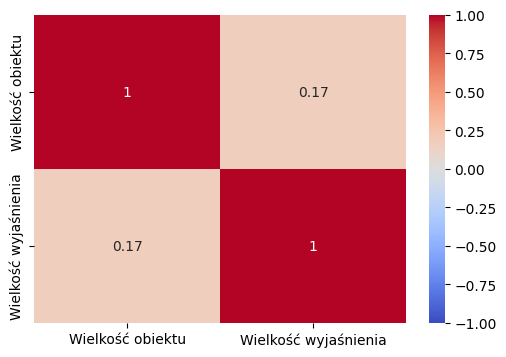
\includegraphics[width=.9\textwidth]{img/size_exp_lime_corr}
	\end{subfigure}
	\caption{Zależność między rozmiarem obiektu, a rozmierem obszaru wyjaśnienia LIME}
\end{figure}
\begin{figure}[h]
	\centering
	\begin{subfigure}[b]{0.45\textwidth}
		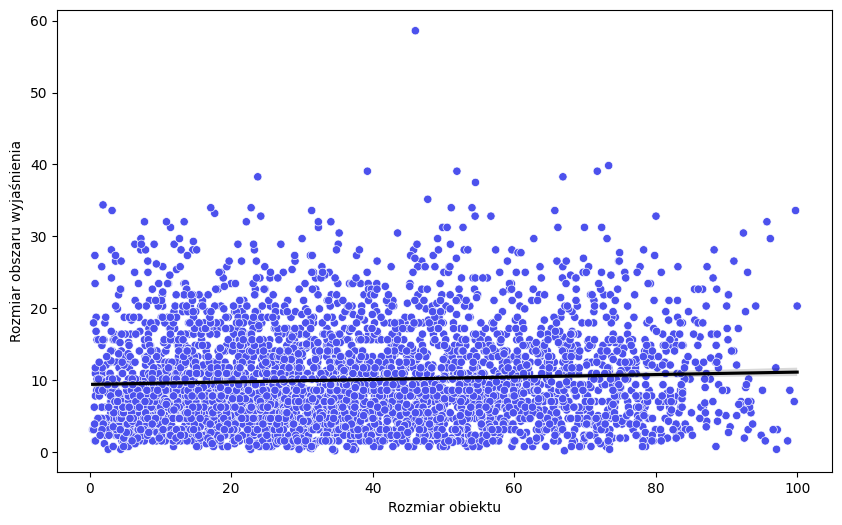
\includegraphics[width=.9\textwidth]{img/size_exp_shap}
	\end{subfigure}
	\begin{subfigure}[b]{0.45\textwidth}
		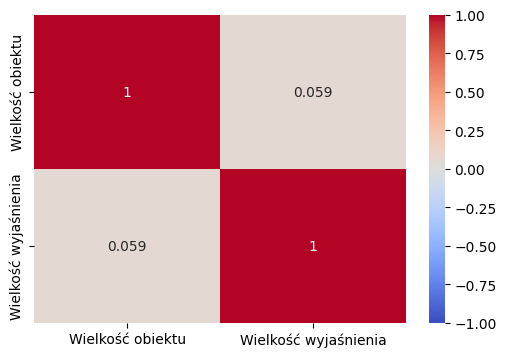
\includegraphics[width=.9\textwidth]{img/size_exp_shap_corr}
	\end{subfigure}
	\caption{Zależność między rozmiarem obiektu, a rozmierem obszaru wyjaśnienia SHAP}
	\label{rys:size_exp_shap}
\end{figure}

Za pomocą wykresów (Rys. \ref{rys:size_exp_gradcam}-\ref{rys:size_exp_shap}) została przedstawiona zależność między rozmiarem a obiektem.

GradCAM wykazał największą korelacje między wielkością obszaru obiektu a wielkością wyjaśnienia.
Na wykresie punktowym (Rys. \ref{rys:size_exp_gradcam}) widoczne jest, że wyjaśnienia GradCAM są ograniczone przez rozmiary ostatniej warstwy konwolucyjnej.

LIME wykazał niższą korelację niż GradCAM.
Dodatkowo wygenerowane wyjaśnienia są zazwyczaj małe, często poniżej 25\% rozmiaru obrazu.
Powodem może być wysoki wpływ dobranych parametrów.

SHAP wykazał najniższą korelacje lub praktycznie jej brak.
Obszary wyjaśnień SHAP są również zazwyczaj mał jak w przypadku LIME.
Może to być również spowodowanie doborem parametrów.

\vspace{1cm}
Analiza wielkości wyjaśnień dla metod GradCAM, LIME i SHAP pokazuje, że każda z tych metod ma różne podejścia do generowania obszarów kluczowych na obrazach.
GradCAM charakteryzuje się największą spójnością wielkości wyjaśnień, odpowiadającej rzeczywistej wielkości obiektów, co może być istotne w zastosowaniach praktycznych.
LIME i SHAP natomiast mniejsze wyjaśnienia, co może być spowodowane doborem parametrów, w celach praktywcznych parametry powinny być dobierane osobno dla każdego przypadku.

